\subsection{Developer Survey}

\begin{frame}
\frametitle{Survey Goals And Population}
\begin{itemize}
\item confirm or deny parts 1 and 2:...
\item investigate some topics: usage freq., pain points, testing, html parsing, ephem vs pers. comparision
\item 18 Dwolla developers, average of 9 years experience
\end{itemize}
\end{frame}
\note[itemize]{
    \item pt 1
    \item pt 2
}
%------------------------------------------------

\begin{frame}
\frametitle{Confirming PT1}
\begin{itemize}
\item idk
\end{itemize}
\end{frame}
\note[itemize]{
    \item pt 1
    \item pt 2
}

%------------------------------------------------

\begin{frame}
\frametitle{Confirming PT2}
\begin{itemize}
\item idk
\end{itemize}
\end{frame}
\note[itemize]{
    \item pt 1
    \item pt 2
}

%------------------------------------------------

\begin{frame}
\frametitle{Regex Testing}
\begin{table}[!htbp]
\centering
\begin{normalsize}
\label{table:codeVsRegexTest}
\caption{\small{Q5: Please describe how often you compose regex for a particular problem type. }}
\begin{tabular}{l|c|c|c|c|c|c|c}
\hline
 & \textbf{Always} & \textbf{V. Freq} & \textbf{Freq.} & \textbf{Occ.} & \textbf{Rarely} & \textbf{V. Rarely} & \textbf{Never} \\
\noalign{\hrule height 0.08em}
test code & 4 & 7 & 5 & 1 & 0 & 0 & 1\\
\hline
test regex & 3 & 4 & 5 & 5 & 1 & 1 & 0\\
\noalign{\hrule height 0.08em}
\end{tabular}
\end{normalsize}
\end{table}

\begin{figure}[ht]
  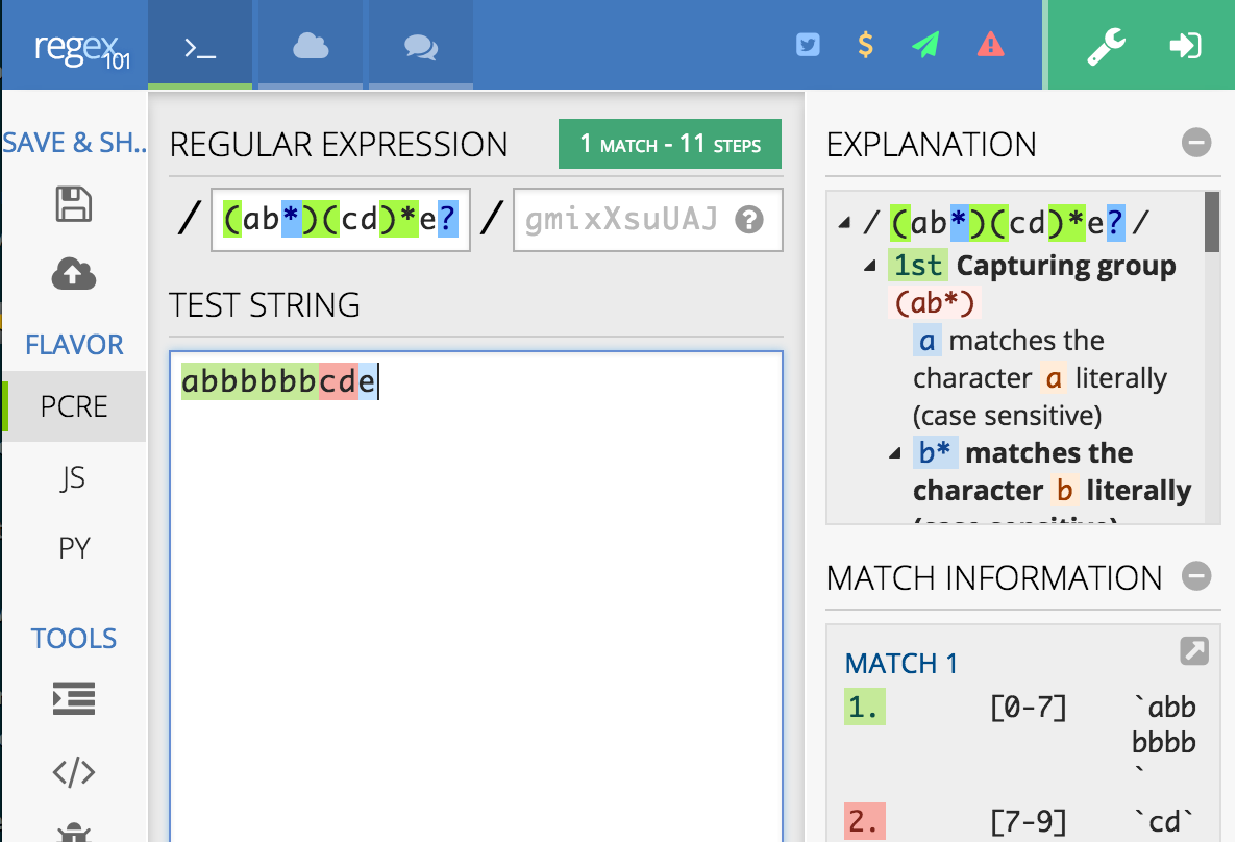
\includegraphics[scale=0.35]{nontex/regex101}
  \label{fig:regex101}
\end{figure}
\begin{center}
50\% say they use testing tools like www.regex101.com
\end{center}
\end{frame}
\note[itemize]{
    \item pt 1
    \item pt 2
}

%------------------------------------------------


\begin{frame}[fragile]
\frametitle{Parsing HTML}
\begin{center}
Only 28\% (5) admit to using regex to parse HTML.
\end{center}
\begin{center}
\cverb!<li><a href="([^"]*)">([^"]*)</a></li>!
\end{center}
\begin{table}
\begin{tabular}{l l l}
\toprule
& \textbf{NParticipants} & \textbf{\%} \\
\midrule
"use only custom parser" & 4 & 22\% \\
"use only regex" & 2 & 11\% \\
"it depends" & 12 & 67\% \\
\bottomrule
\end{tabular}
\caption{Would you rather use regex or a custom parser?  }
\begin{block}{If it depends, why?}
\emph{parsers are more powerful than regex, if the problem can be solved with regex I prefer regex...}
\\* \emph{If this is a one off application than a regex will work fine.}
\end{block}
\end{table}

\end{frame}
\note[itemize]{
    \item Of those who said it depends, there was much agreement that parsers are more powerful, better at handling complexity, and provide more readable code. Regexes were mentioned positively for handling less structured inputs, form validation and ‘one-off’ programs
}

%------------------------------------------------

\begin{frame}
\frametitle{Usage Frequency - By Technical Environment}
\begin{center}
Heaviest regex use is in Command line tools and text editors.
\end{center}
\begin{adjustbox}{width=\textwidth}
\begin{tabular}{l | r @{  } r @{  } r @{  } r @{  } r @{  } r }
\toprule
\textbf{Language/Environment} & \textbf{0} & \textbf{1-5} & \textbf{6-10} & \textbf{11-20} & \textbf{21-50} & \textbf{51+} \\  \midrule
General  (e.g., Java)  & 1 & 6 & 5 & 3& 1& 2 \\ \midrule
Scripting  (e.g., Perl) &5 &4 &3 &3 &2  &1 \\ \midrule
Query  (e.g., SQL) & 15&2 &0 &0 &1  & 0\\ \midrule
Command line (e.g., grep)   &2 &5 &3 &2 &0  &\textcolor{red}{6} \\ \midrule
Text editor (e.g., IntelliJ)   & 2& 5& 0& 5& 1& \textcolor{red}{5}\\
\bottomrule
\end{tabular}
\end{adjustbox}

\end{frame}
\note[itemize]{
    \item Only 27\% (5) of participants wrote regular expressions that persist (general purpose, scripting, etc.) more frequently than in a text editor or command line tool (where they will not persist).
}

%------------------------------------------------


\begin{frame}
\frametitle{Ephemeral vs Persistent Users}
\begin{adjustbox}{width=\textwidth}
\begin{tabular}{lccc}
\toprule
\textbf{Task} & \textbf{Persistence Freq.} & \textbf{Ephemeral Freq.} & \textbf{Difference} \\  \midrule
Counting  substrings that match a pattern & 3 & 1.7 & 1.2\\  \midrule
Parsing user input & 3.6 & 2.7 & 0.9\\ \midrule
Capturing parts of strings & 3.8 & 3.1 & 0.7\\ \midrule
Parsing generated text & 2.4 & 1.9 & 0.5\\  \midrule
Locating content within a file or files & 3.6 & 3.2 & 0.4\\ \midrule
Filtering collections (lists, tables, etc.) & 2.2 & 1.9 & 0.3\\ \midrule
Counting lines that match a pattern & 1.8 & 2.1 & -0.3\\
\bottomrule
\end{tabular}
\end{adjustbox}

\begin{table}
\caption{Survey results for regex usage frequencies, comparing persistent and ephemeral users \label{table:persistingFeatureGroups}}
\begin{center}
\begin{small}
\begin{tabular}{llccc}
\toprule
\textbf{Group} & \textbf{Code} &  \textbf{Ephemeral Users} & \textbf{Persistent Users} & \textbf{Difference}\\  \midrule \bigstrut
\multirow{2}{*}{(neg) look-ahead/behind} &  (LKA, NLKA,  & \multirow{2}{*}{2.2} & \multirow{2}{*}{3.2} & \multirow{2}{*}{1.0} \\
& LKB, NLKB) & &\\
\midrule \bigstrut
lazy repetition & (LZY) &  2.8 & 3 & 0.2\\
\midrule \bigstrut
endpoint anchors & (STR, END) & 4.4 & 4.4 & 0\\ \midrule \bigstrut
capture groups & (CG) & 4.2 & 4.2 & 0\\ \midrule \bigstrut
word boundaries & (WNW) & 3.5 & 3.4 & -0.1\\
\bottomrule
\end{tabular}
\end{small}
\end{center}
\vspace{-12pt}
\end{table}

\end{frame}
\note[itemize]{
    \item The five persistent users have an average of 12.4 years of experience. This contrasts with an average of 7.7 years of experience for ephemeral users. Considering usage frequency, 60\% (3) of the five persistent users indicate using regex weekly, vs 46\% (6) of the 13 ephemeral users.
    \item In the case of the most rarely-used feature asked about, the OPT feature, three of the four participants who have ever used the OPT feature are persistent users
}

%------------------------------------------------

\begin{frame}
\frametitle{Pain Points}
\begin{block}{hard to compose (11)}
\emph{...very difficult to write them since I`ve never read up on them.}
\\*\emph{...trickiness to getting the expression right}
\end{block}
\begin{block}{hard to read (7)}
\emph{long ones can be hard to read}
\\*\emph{Readability. Edge cases.}
\\*\emph{It is terrible to read (especially later after initial development) }
\end{block}
\begin{block}{inconsistency across implementations (3)}
\emph{Differences in implementation across languages}
\\*\emph{Some regexes work differently (or don`t work) in some languages.}
\end{block}
\end{frame}
\note[itemize]{
    \item pt 1
    \item pt 2
}

%------------------------------------------------











